% Compile: pdflatex projection_head_explained.tex   (run twice for references)
% Standard packages only: amsmath, amssymb, booktabs, geometry, tikz.
\documentclass[11pt]{article}
\usepackage{amsmath,amssymb,bm}
\usepackage[margin=2.6cm]{geometry}
\usepackage{booktabs}
\usepackage{tikz}
\usepackage[colorlinks=true,linkcolor=black,citecolor=black]{hyperref}

\newcommand{\s}{\mathbf{s}}
\newcommand{\F}{\mathbf{F}}
\newcommand{\Pv}{\mathbf{P}}
\newcommand{\lo}{\bm{\ell}}
\newcommand{\hi}{\mathbf{u}}
\newcommand{\R}{\mathbb{R}}

\title{From the network to a feasible dispatch\\
\large What the projection head does, built up from two dimensions}
\author{}
\date{}

\begin{document}
\maketitle

\noindent
The network emits a vector of numbers. Those numbers are almost never a legal
dispatch: they do not meet demand, they may be negative, they may exceed what a
plant can produce, and they may jump faster than a plant can ramp. The
\emph{projection head} turns them into the closest legal dispatch. This note
builds that map from the smallest case upward, using nothing beyond a first
course in linear algebra, and finishes on a real step from the trained model.

Sections \ref{sec:two}--\ref{sec:box} are illustrative numbers chosen to be easy
to check by hand. Section~\ref{sec:real} is a genuine step, values taken
straight from the model.

\tableofcontents

% ============================================================
\section{Two channels, one equation}
\label{sec:two}

Suppose the fleet has just two plants, coal and hydro, and write their outputs
as a vector in $\R^2$:
\[
  \Pv = \begin{pmatrix} P_1 \\ P_2 \end{pmatrix}
      = \begin{pmatrix} \text{coal} \\ \text{hydro}\end{pmatrix}\ \text{MW}.
\]
Demand is $d = 1000$ MW and both plants generate, so the rule is
\[
  \boxed{\;P_1 + P_2 = 1000\;}
\]
Write $\s = (1,1)^{\!\top}$. The rule is the single linear equation
$\s^{\!\top}\Pv = d$, and its solution set
\[
  H \;=\; \{\, \mathbf{x}\in\R^2 \;:\; \s^{\!\top}\mathbf{x} = d \,\}
\]
is a \textbf{line} in the plane, with $\s$ as its normal vector. Every legal
dispatch lies on that line.

Now suppose the network proposes
\[
  \F = \begin{pmatrix} 700 \\ 400 \end{pmatrix},
  \qquad \s^{\!\top}\F = 1100 \neq 1000 .
\]
It oversupplies by $100$ MW. We want the point of $H$ closest to $\F$:
\[
  \Pv^\star \;=\; \arg\min_{\Pv \in H} \ \lVert \Pv - \F \rVert^2 .
\]

\subsection*{Careful: this is not $\mathrm{proj}_{\mathbf{u}}(\mathbf{v})$}

A first course gives you the projection of one vector onto another,
\[
  \mathrm{proj}_{\mathbf{u}}(\mathbf{v})
  \;=\; \frac{\mathbf{u}^{\!\top}\mathbf{v}}{\mathbf{u}^{\!\top}\mathbf{u}}\,\mathbf{u},
\]
which lands on $\mathrm{span}(\mathbf{u})$ --- a line \emph{through the origin},
i.e.\ a subspace. That is not our situation. Our set is
$H = \{\mathbf{x} : \s^{\!\top}\mathbf{x} = 1000\}$, which does not contain the
origin, so $H$ is not a subspace at all; it is an \textbf{affine} hyperplane. And
we want the closest point of $H$ itself, not of $\mathrm{span}(\s)$.

The standard formula still does the work, one level down. Pick any
$\mathbf{x}_0 \in H$ and write $H = \mathbf{x}_0 + H_0$, where
\[
  H_0 \;=\; \{\mathbf{x} : \s^{\!\top}\mathbf{x} = 0\} \;=\; \s^{\perp}
\]
\emph{is} a subspace. Projecting onto an affine set means: shift to the origin,
project onto the subspace, shift back. Projecting onto $\s^{\perp}$ is removing
the component along $\s$, which is exactly $\mathbf{y} - \mathrm{proj}_{\s}(\mathbf{y})$.
So
\begin{align*}
  \Pi_H(\F)
  &= \mathbf{x}_0 + \Pi_{H_0}\!\left(\F - \mathbf{x}_0\right) \\
  &= \mathbf{x}_0 + (\F - \mathbf{x}_0) - \mathrm{proj}_{\s}(\F - \mathbf{x}_0)
     \qquad \text{\small ($\mathrm{proj}_{\s}$ enters here, on the \emph{offset})} \\
  &= \F - \frac{\s^{\!\top}(\F - \mathbf{x}_0)}{\s^{\!\top}\s}\,\s \\
  &= \F - \frac{\s^{\!\top}\F - d}{\lVert\s\rVert^{2}}\,\s
     \qquad \text{\small (since $\s^{\!\top}\mathbf{x}_0 = d$)}
\end{align*}
The arbitrary choice of $\mathbf{x}_0$ cancels, which is why the answer ends up
looking so much like the subspace formula. Writing the correction as
$\lambda\s$:
\[
  \boxed{\;\Pv^\star = \F + \lambda\s,
  \qquad \lambda \;=\; \frac{d - \s^{\!\top}\F}{\lVert\s\rVert^{2}}\;}
\]

\paragraph{Two checks.} The answer satisfies the rule,
\[
  \s^{\!\top}\Pv^\star = \s^{\!\top}\F + \lambda\lVert\s\rVert^{2}
                       = \s^{\!\top}\F + d - \s^{\!\top}\F = d,
\]
and the distance travelled,
$\lVert \Pv^\star - \F\rVert = \lvert \s^{\!\top}\F - d\rvert / \lVert\s\rVert$,
is the familiar point-to-hyperplane distance.

\paragraph{The same thing in one line.} You can also just \emph{assume} the
answer has the form $\Pv = \F + \lambda\s$ --- move along the normal until you
hit the plane --- and solve $\s^{\!\top}(\F + \lambda\s) = d$ for the single
unknown $\lambda$. That is the derivation used from Section~\ref{sec:box}
onward, where a box makes the geometric route messier but the ``one unknown
$\lambda$'' route still works.

Two things are worth naming right away, because they carry all the way to the
real model.

\begin{itemize}
\item Define the \textbf{balance gap} $\Delta = d - \s^{\!\top}\F$. Here
      $\Delta = -100$: the guess supplies $100$ MW too much.
\item Every entry of $\s$ is $\pm 1$, so $\lVert\s\rVert^2 = n$, the number of
      channels. Here $n=2$.
\end{itemize}

So $\lambda = -100/2 = -50$ and
\[
  \Pv^\star = \begin{pmatrix}700\\400\end{pmatrix}
            + (-50)\begin{pmatrix}1\\1\end{pmatrix}
            = \begin{pmatrix}650\\350\end{pmatrix},
  \qquad 650 + 350 = 1000 .\ \checkmark
\]

\begin{center}
% unit vectors, not \scale -- so node text keeps its normal size
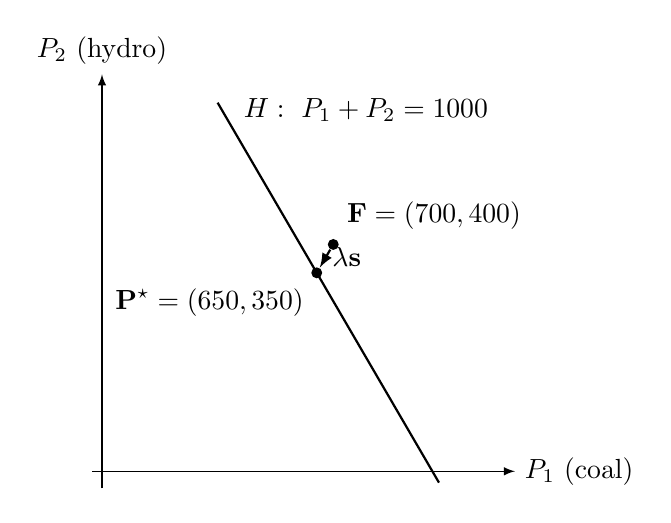
\begin{tikzpicture}[x=0.0042cm, y=0.0072cm, >=latex,
                    dot/.style={circle, fill, inner sep=1.4pt}]
  \draw[->] (-30,0) -- (1250,0) node[right] {$P_1$ (coal)};
  \draw[->] (0,-30) -- (0,700) node[above] {$P_2$ (hydro)};
  \draw[thick] (350,650) -- (1020,-20);
  \node[anchor=south west] at (400,600) {$H:\ P_1+P_2=1000$};
  \node[dot] (F) at (700,400) {};
  \node[anchor=south west] at (712,410) {$\F=(700,400)$};
  \node[dot] (P) at (650,350) {};
  \node[anchor=north east] at (640,340) {$\Pv^\star=(650,350)$};
  \draw[->, thick] (F) -- (P);
  \node[anchor=west] at (668,378) {$\lambda\s$};
\end{tikzpicture}
\end{center}

\medskip
\noindent\textbf{Read the answer.} The $100$ MW of oversupply was removed by
taking $50$ MW off \emph{each} channel. Nothing in the problem said anything
about coal being large and hydro being small; the squared distance
$\lVert\Pv-\F\rVert^2$ treats both coordinates identically, so the correction
splits evenly. Remember this --- it is the defect we fix in
Section~\ref{sec:weights}.

% ============================================================
\section{A channel that consumes: the sign vector}

A battery charging is a \emph{load}, not a source. If channel 2 is charging,
supply is $P_1 - P_2$ and the rule becomes
\[
  P_1 - P_2 = d, \qquad \s = \begin{pmatrix}1\\-1\end{pmatrix}.
\]
Nothing about the derivation changes: $\lVert\s\rVert^2 = 1 + (-1)^2 = 2$ still,
because squaring kills the sign. With $d=1000$ and
$\F = (1100,\ 50)^{\!\top}$ we get $\s^{\!\top}\F = 1050$, $\Delta = -50$,
$\lambda = -25$, and
\[
  \Pv^\star = \begin{pmatrix}1100\\50\end{pmatrix} + (-25)\begin{pmatrix}1\\-1\end{pmatrix}
            = \begin{pmatrix}1075\\75\end{pmatrix},
  \qquad 1075 - 75 = 1000 .\ \checkmark
\]
Generation went \emph{down} by 25 and charging went \emph{up} by 25. Both
changes reduce net supply, which is what $\Delta<0$ asked for. The $-1$ entry
made the second channel move the opposite way automatically.

This is the sign vector used in the real model, with charging as the one
negative entry:
\[
  \s = (\,\underbrace{1}_{\text{hydro}},\ \underbrace{1}_{\text{coal}},\
        \underbrace{1}_{\text{gas steam}},\ \underbrace{1}_{\text{gas OCGT}},\
        \underbrace{-1}_{\text{batt.\ charge}},\ \underbrace{1}_{\text{batt.\ discharge}}\,)^{\!\top}.
\]

% ============================================================
\section{Three channels, and a box}
\label{sec:box}

Plants also have limits. A plant cannot go below zero, cannot exceed its
capacity, and cannot move further than its ramp rate in one five-minute step.
Once the previous step is fixed, \emph{every one of those limits is just a lower
and an upper number per channel} --- we build them explicitly in
Section~\ref{sec:ramp}. For now take them as given:
\[
  B \;=\; \{\,\mathbf{x} : \ell_i \le x_i \le u_i \ \ \text{for all } i \,\}
\]
a \textbf{box} (an axis-aligned rectangle). The feasible set is now
\[
  C \;=\; H \cap B,
\]
a line segment in $\R^2$, a convex polygon in $\R^3$, and in general the
intersection of a hyperplane with a box. It is convex, which is why a unique
closest point exists.

Take three channels, $\s = (1,1,1)^{\!\top}$, $d = 1000$, and
\[
  \F = \begin{pmatrix}700\\250\\120\end{pmatrix}
  \quad(\text{coal, hydro, gas}), \qquad \s^{\!\top}\F = 1070,\quad \Delta = -70 .
\]
The unconstrained answer from Section~\ref{sec:two} is $\lambda = -70/3 =
-23.33$, giving
\[
  \F + \lambda\s = (676.67,\ 226.67,\ 96.67)^{\!\top}.
\]
Suppose gas cannot fall below $\ell_3 = 100$ MW this step, because it was at
$140$ and its down-ramp is $40$. Then $96.67$ is illegal.

\subsection*{The shape of the answer}

Clamp the offending coordinate and re-solve. The correct general form is
\[
  \boxed{\;\Pv^\star \;=\; \mathrm{clip}\bigl(\F + \lambda\s,\ \lo,\ \hi\bigr)\;}
\]
for a \emph{single} scalar $\lambda$, where $\mathrm{clip}$ acts coordinatewise.
The picture: you still travel along the normal $\s$, but each coordinate stops
when it hits its wall. Coordinates strictly inside the box behave as though only
the equation existed; coordinates pressed against a wall are frozen.

Call $A$ the \textbf{active set} --- the coordinates that end up strictly inside
(``free''). For $i \in A$ we have $P_i = F_i + \lambda s_i$, so
$s_i P_i = s_i F_i + \lambda s_i^2 = s_i F_i + \lambda$. Summing the balance
equation over frozen and free parts,
\[
  d \;=\; \underbrace{\sum_{i \notin A} s_i P_i}_{\text{fixed at a wall}}
        \;+\; \sum_{i \in A}\bigl(s_i F_i + \lambda\bigr)
\]
and therefore
\begin{equation}
\boxed{\;
  \lambda \;=\;
  \frac{\,d \;-\; \sum_{i \notin A} s_i P_i \;-\; \sum_{i \in A} s_i F_i\,}{\lvert A\rvert}\;}
\label{eq:lambda}
\end{equation}
Once you know \emph{which} coordinates are stuck, $\lambda$ is one division.

\subsection*{Back to the numbers}

Gas is frozen at $P_3 = 100$, so $A = \{1,2\}$, $\lvert A\rvert = 2$, and
\[
  \lambda = \frac{1000 - 100 - (700+250)}{2} = \frac{-50}{2} = -25 .
\]
\[
  \Pv^\star = (700-25,\ \ 250-25,\ \ 100)^{\!\top} = (675,\ 225,\ 100)^{\!\top},
  \qquad 675+225+100 = 1000 .\ \checkmark
\]
Note $\lambda$ moved from $-23.33$ to $-25$: with gas unable to take its share,
the other two absorb more.

\subsection*{Why there is exactly one $\lambda$}

Equation~\eqref{eq:lambda} presumes we know $A$. Finding $A$ is the only
combinatorial part, and it is easy because the problem is monotone. Define
\[
  g(\lambda) \;=\; \s^{\!\top}\,\mathrm{clip}(\F + \lambda\s,\ \lo,\ \hi).
\]
Differentiate coordinate $i$'s contribution:
\[
  \frac{d}{d\lambda}\Bigl[s_i\,\mathrm{clip}(F_i + \lambda s_i,\ \ell_i, u_i)\Bigr]
  \;=\;
  \begin{cases}
    s_i^2 = 1, & \text{if coordinate $i$ is free,}\\[2pt]
    0, & \text{if it is clamped.}
  \end{cases}
\]
Because every $s_i = \pm 1$, the square erases the sign: \textbf{every free
coordinate pushes $g$ in the same direction.} The $-1$ on battery charging
cannot cancel a $+1$ elsewhere. Hence $g$ is piecewise linear and
non-decreasing, with slope exactly $\lvert A\rvert$, so the equation
$g(\lambda) = d$ has a unique solution (up to a flat segment) and a bisection
finds it. In the code this is a $40$--$60$ step bisection under
\texttt{no\_grad}, used \emph{only} to identify $A$; the returned value is then
recomputed by \eqref{eq:lambda}, which is differentiable in $\F$ so the network
can be trained through the layer.

% ============================================================
\section{Weighting: who should absorb the correction}
\label{sec:weights}

Section~\ref{sec:two} ended on a complaint. Minimising
$\lVert\Pv-\F\rVert^2$ moves every free channel by the same number of megawatts.
In the real fleet that is wrong: gas steam has a $516$ MW cap and is switched off
most of the time, while brown coal has a $4{,}896$ MW cap and is almost always
the marginal unit. An equal split hands them the same correction.

Fix it by minimising a \textbf{weighted} distance:
\[
  \Pv^\star \;=\; \arg\min_{\Pv \in C} \ \sum_{i} w_i \,(P_i - F_i)^2,
  \qquad w_i > 0 .
\]
Redo the derivation. Ignoring the box, the Lagrangian is
$\tfrac12\sum_i w_i (P_i-F_i)^2 - \lambda(\s^{\!\top}\Pv - d)$ and setting the
gradient to zero gives $w_i (P_i - F_i) - \lambda s_i = 0$, i.e.
\[
  \boxed{\;P_i \;=\; F_i + \lambda \frac{s_i}{w_i}\;}
\]
Same shape, one scalar, travel direction rescaled per coordinate. Substituting
into $\s^{\!\top}\Pv = d$:
\[
  d \;=\; \s^{\!\top}\F + \lambda \sum_i \frac{s_i^2}{w_i}
      \;=\; \s^{\!\top}\F + \lambda \sum_i \frac{1}{w_i}
  \qquad\Longrightarrow\qquad
  \lambda \;=\; \frac{\Delta}{\sum_i 1/w_i}.
\]
Everything from Section~\ref{sec:box} survives: $g$ is still monotone (a free
coordinate now contributes slope $1/w_i > 0$ instead of $1$), so bisection still
works, and \eqref{eq:lambda} becomes
\begin{equation}
  \lambda \;=\;
  \frac{\,d - \sum_{i\notin A} s_i P_i - \sum_{i\in A} s_i F_i\,}
       {\sum_{i \in A} 1/w_i}.
\label{eq:lambdaw}
\end{equation}

\subsection*{The weights are the merit order}

Here is the payoff. How much of the correction does channel $i$ take? Its signed
contribution is
\[
  s_i \,\Delta P_i \;=\; s_i \cdot \lambda\frac{s_i}{w_i} \;=\; \frac{\lambda}{w_i},
  \qquad\text{and}\qquad
  \sum_i s_i \Delta P_i = \Delta,
\]
so the \textbf{share} channel $i$ absorbs is
\[
  \boxed{\;
  \frac{s_i\,\Delta P_i}{\Delta} \;=\; \frac{1/w_i}{\sum_j 1/w_j} \;=:\; p_i \;}
\]
a genuine probability distribution over the channels. Inverting: choosing
$w_i = 1/p_i$ makes channel $i$ absorb exactly the share $p_i$.

\medskip\noindent
\textbf{Worked check.} Three channels again, $\Delta = -70$, and suppose coal
should resist moving ten times as much as the others: $\mathbf{w} = (10,1,1)$.
Then $\sum_i 1/w_i = 0.1 + 1 + 1 = 2.1$ and $\lambda = -70/2.1 = -33.33$, giving
\[
  \Delta\Pv = \lambda\Bigl(\tfrac{1}{10},\ 1,\ 1\Bigr)
            = (-3.33,\ -33.33,\ -33.33)^{\!\top},
\]
so coal takes $3.33/70 = 4.76\%$ of the correction, which is exactly
$(1/10)/2.1$. \checkmark

\medskip\noindent
In the model, $p$ is not written down by hand: the network emits six extra
numbers per step and $p = \mathrm{softmax}(\text{logits})$. Softmax is the
natural parameterisation because $p$ \emph{must} be a distribution, and softmax
cannot emit anything else --- so the network can no more propose an inconsistent
split than the projection can emit an infeasible dispatch.

Crucially, none of the guarantees depend on $w$. For \emph{any} positive $w$ the
output still satisfies the balance equation exactly and still lies in the box.
The weights change only \emph{where} the correction lands.

% ============================================================
\section{Ramps: turning a trajectory into a box}
\label{sec:ramp}

So far one time step. The real task fills a gap of $N = 36$ consecutive
five-minute steps, and ramp limits tie neighbours together:
\[
  -r^{\mathrm{dn}}_i \;\le\; P_{j,i} - P_{j-1,i} \;\le\; r^{\mathrm{up}}_i .
\]
That is $36 \times 6 = 216$ variables coupled across time --- not a
per-step problem at all. The head decouples it by sweeping forward: solve step
$1$, fix it, solve step $2$, and so on. \textbf{Once $\Pv_{j-1}$ is a fixed
vector of numbers, every constraint on step $j$ collapses into a lower and an
upper bound per channel:}
\[
\boxed{
\begin{aligned}
  \ell_{j,i} &= \max\bigl(\,0,\ \ P_{j-1,i} - r^{\mathrm{dn}}_i,\ \
                   p^R_i - k\,r^{\mathrm{up}}_i \,\bigr)\\[2pt]
  u_{j,i}    &= \min\bigl(\,\mathrm{cap}_i,\ \ P_{j-1,i} + r^{\mathrm{up}}_i,\ \
                   p^R_i + k\,r^{\mathrm{dn}}_i \,\bigr)
\end{aligned}}
\qquad k = N + 1 - j
\]
Three terms each, and they are worth reading separately.

\begin{enumerate}
\item $0$ and $\mathrm{cap}_i$: the plant's physical floor and ceiling.
\item $P_{j-1,i} \pm r_i$: it cannot move faster than its ramp rate.
\item $p^R_i \mp k\,r_i$: \textbf{backward reachability}. The gap has a pinned
      right-hand boundary $\mathbf{p}^R$ --- the observed dispatch at the far
      side. With $k$ steps remaining you can climb at most $k\,r^{\mathrm{up}}_i$,
      so you must already be at least $p^R_i - k\,r^{\mathrm{up}}_i$ or you can
      never arrive. Symmetrically for the descent.
\end{enumerate}

Term 3 is what makes the greedy sweep safe. Without it a locally optimal early
step could strand the trajectory somewhere it cannot return from; with it, one
shows by induction on $j$ that $[\lo_j, \hi_j]$ is never empty. So the whole
$216$-dimensional coupled problem becomes $36$ independent six-dimensional
projections of exactly the kind built in Sections~\ref{sec:box}
and~\ref{sec:weights}.

\medskip\noindent
\textbf{Where exactness can still fail.} The box is guaranteed non-empty; its
intersection with the hyperplane is not. The attainable range of
$\s^{\!\top}\Pv$ over the box is
\[
  \Bigl[\ \textstyle\sum_i \min(s_i\ell_i,\ s_iu_i),\ \ \sum_i \max(s_i\ell_i,\ s_iu_i)\ \Bigr],
\]
and if $d$ falls outside it, no legal dispatch meets demand at that step. The
projection then returns the nearest attainable point and reports the shortfall.
Measured on $400$ test windows ($14{,}400$ steps) under the current envelope, the
box admits a range of mean width $3{,}691$ MW and $d$ sits at least $431$ MW from
the nearer end at the tightest step, so this never occurs --- but it is a
property of the data, not a theorem.

% ============================================================
\section{A real step}
\label{sec:real}

Everything above, on genuine values from the trained \texttt{hardnet\_alloc}
model, first step of one test gap. Units are MW.

\[
  \s = (1,\ 1,\ 1,\ 1,\ -1,\ 1)^{\!\top}, \qquad n = 6 .
\]

\begin{center}
\small
\begin{tabular}{lrrrrrr}
\toprule
 & hydro & coal & gas steam & gas OCGT & batt.\ chg & batt.\ dis \\
\midrule
$\mathbf{p}^L$ (pinned left)   &  733.0 & 3681.5 &  97.1 &  701.0 &  99.6 & 19.5 \\
$\mathbf{p}^R$ (pinned right)  &  620.0 & 3595.9 &  99.8 &  607.7 & 885.8 &  0.0 \\
\midrule
$\F$ \emph{(network guess)}    &  743.5 & 3716.9 & 138.6 &  736.1 &  88.2 & $-12.6$ \\
$\mathbf{p}$ \emph{(network split)} & 0.244 & 0.031 & 0.185 & 0.250 & 0.145 & 0.145 \\
$\mathbf{w} = 1/\mathbf{p}$    &   4.1 &   32.0 &   5.4 &    4.0 &   6.9 &  6.9 \\
\midrule
$\lo$ (box lower)              &    0.0 & 3538.5 &  56.2 &  337.1 &   0.0 &  0.0 \\
$\hi$ (box upper)              & 1689.5 & 3828.9 & 128.6 & 1101.3 & 894.6 & 734.5 \\
\midrule
$\Pv^\star$ \emph{(output)}    &  671.9 & 3707.8 &  84.4 &  663.3 & 130.8 &  0.0 \\
\bottomrule
\end{tabular}
\end{center}

\paragraph{Step 1 --- the gap.} Net demand at this step is $d = 4996.6$, while
\[
  \s^{\!\top}\F = 743.5 + 3716.9 + 138.6 + 736.1 - 88.2 + (-12.6) = 5234.3,
\]
so $\Delta = d - \s^{\!\top}\F = -237.7$. The guess oversupplies by $237.7$ MW.
Note also that the network proposed $-12.6$ MW of battery discharge, which is
physically impossible; the box will deal with it.

\paragraph{Step 2 --- which coordinates are free.} The bisection finds that five
channels land strictly inside their box and battery discharge is driven below
its floor and clamps at $0$. So
\[
  A = \{\text{hydro, coal, gas steam, gas OCGT, batt.\ chg}\},
  \qquad
  \sum_{i\in A}\frac{1}{w_i} = 0.8544 .
\]

\paragraph{Step 3 --- the multiplier.} By \eqref{eq:lambdaw}, with the one
clamped channel contributing $s_i P_i = 0$:
\[
  \lambda = \frac{4996.6 - 0 - \bigl(743.5+3716.9+138.6+736.1-88.2\bigr)}{0.8544}
          = \frac{-250.3}{0.8544} = -292.9 .
\]

\paragraph{Step 4 --- the moves.} $\Delta P_i = \lambda s_i / w_i$:
\begin{center}
\small
\begin{tabular}{lrrr}
\toprule
channel & $\lambda s_i / w_i$ & result & note \\
\midrule
hydro        & $-292.9/4.1  = -71.4$ &  671.9 & \\
coal         & $-292.9/32.0 = \ \ -9.2$ & 3707.8 & barely moves: $w=32$, i.e.\ $p=0.031$ \\
gas steam    & $-292.9/5.4  = -54.2$ &   84.4 & \\
gas OCGT     & $-292.9/4.0  = -73.2$ &  663.3 & \\
batt.\ chg   & $+292.9/6.9  = +42.5$ &  130.8 & \emph{rises} --- $s_i=-1$, charging more cuts net supply \\
batt.\ dis   & $-292.9/6.9  = -42.5$ &    0.0 & would give $-55.2$; clipped at the floor \\
\bottomrule
\end{tabular}
\end{center}

\paragraph{Step 5 --- verify.}
\[
  \s^{\!\top}\Pv^\star = 671.9 + 3707.8 + 84.4 + 663.3 - 130.8 + 0.0
  = 4996.6 = d .\ \checkmark
\]
Every entry lies in $[\lo,\hi]$ by construction, since the last operation is a
clip into that interval. Audited over ten counterfactual days, the worst balance
residual across all steps is $8\times10^{-4}$ MW on a $5$ GW stack --- float32
rounding, not solver error.

\paragraph{What the weights bought.} Under the unweighted head ($w_i \equiv 1$)
the same $\Delta$ would have been split equally, $-237.7/6 = -39.6$ MW on every
channel, including coal. The learned split moved coal only $9.2$ MW and put the
correction on hydro and OCGT instead. Whether that particular call is right is a
question about the model; the point here is that it is now \emph{the model's
call}, and it used to be arithmetic.

% ============================================================
\section*{Summary}
\addcontentsline{toc}{section}{Summary}

\begin{enumerate}
\item One linear equation defines a hyperplane; its normal is the sign vector
      $\s$. Projecting onto it is $\Pv = \F + \lambda\s$ with
      $\lambda = \Delta / \lVert\s\rVert^2$.
\item Adding a box keeps the same shape,
      $\Pv = \mathrm{clip}(\F + \lambda\s, \lo, \hi)$; only $\lambda$ must be
      re-solved. It is unique because $s_i^2 = 1$ makes the balance sum
      monotone in $\lambda$.
\item Weighting the distance rescales the travel direction to $\s/\mathbf{w}$
      and nothing else. The share each channel absorbs is
      $(1/w_i)/\sum_j (1/w_j)$, so $w = 1/p$ delivers the split $p$.
\item Ramps and the pinned right boundary are folded into $\lo$ and $\hi$ by a
      forward sweep with a reachability guard, turning $216$ coupled variables
      into $36$ six-dimensional projections.
\item Feasibility holds for any $w$. Letting the network emit $p$ therefore
      makes the allocation learned at no cost to the guarantee.
\end{enumerate}

\end{document}
